\documentclass[11pt]{article}

\usepackage[utf8]{inputenc}
\usepackage[T1]{fontenc}
\usepackage{amsmath,amssymb}
\usepackage{booktabs}
\usepackage{graphicx}
\usepackage{hyperref}
\usepackage[margin=1in]{geometry}
\usepackage{url}
\def\UrlBreaks{\do\/\do-\do_}

\hypersetup{colorlinks=true, linkcolor=blue, citecolor=blue, urlcolor=blue}
\setlength{\tabcolsep}{4pt}

\title{When a Quantum Compiler Looks Like a Better Learner:\\
Confounds in Quantum Machine Learning Comparisons}

\author{TN Holdings\\
\texttt{love.os.architect@proton.me}\\
\texttt{https://github.com/TN-Holdings-LLC/psf-zero}}

\date{Version 1.2 --- 25 October 2026}

\begin{document}
\maketitle

\begin{abstract}
PSF-Zero places a quantum classifier's entangling ring on hardware by formula, without a layout search and without
reading the day's calibration; Qiskit's preset pass manager searches, using the calibration. We ask which of the two
gives the better trained classifier, and report what it took to answer that question honestly. The model is a
10-qubit, 16-layer data re-uploading classifier trained by a finite-difference optimiser on a noise model of
\texttt{ibm\_marrakesh} (the \emph{twin}) and tested on an independently perturbed noise model (the \emph{stand-in});
one day of hardware runs is included. Four effects can each produce a winner without any difference in learning:
(i) the task's answer sat at the untrained starting point --- on the device day's task the untrained model is already
$0.934$ accurate (noiseless), and training lowered both compilers' models to $0.762$ (PSF-Zero) and $0.730$ (Qiskit);
(ii) a readout offset makes a circuit answer one class on $84$--$94\,\%$ of balanced test points, which moves accuracy
while leaving the model unchanged; (iii) arms with different output scales lose different amounts to a fixed shot
count; (iv) the twin's scale was off by up to $2.3\times$ on hardware. With the task moved far from the start and the
rules fixed before each run, PSF-Zero's newest ring schedule (the \emph{zipper}, $336$ CZ and $11.7\,\mu$s at 16
layers) and Qiskit ($506$ CZ, $48.2\,\mu$s, $14$ active qubits) gave classifiers that the declared tests could not tell
apart: on stand-in accuracy the zipper won on one of three teachers at each budget, below the declared two of
three, and on the trained model itself neither arm won on any teacher. Formula placement could not be told apart from the search while using a third fewer entangling gates and a
quarter of the duration; it did not beat it. In one preliminary hardware job on \texttt{ibm\_kingston}, the zipper's
circuits followed a twin built from that day's calibration (scale $1.00$, correlation $0.98$), while Qiskit's lost most
of their signal and came out inverted on the read-out qubit; the cause is not known. We give the vanity and the essential number side by side throughout, mark what was
declared before the data and what was found after, and close with a checklist for compiler comparisons through
trained quantum models.
\end{abstract}

\section{Introduction}

A compiler for near-term quantum hardware is usually judged on circuit metrics: two-qubit gate count, depth, duration,
estimated success probability. The users of a variational quantum classifier care about something else: whether the
trained model is better. Comparing compilers through a trained model is tempting, because it measures what users
want, and dangerous, because training, readout and finite sampling each add their own ways for one arm to win.

The question behind this study is the design question of PSF-Zero~\cite{psfzero}. Its AI front end places the
classifier's ring of CZ gates on a heavy-hex line by a closed formula and routes it with a fixed schedule; it does not
search over layouts and does not read the day's calibration. Qiskit~\cite{qiskit} at optimisation level 2 with the
device's \texttt{Target} searches for a layout and routing, and its choices use the calibrated error rates. A formula
gives a shorter, reproducible circuit; a search can pick better qubits. Which gives the better classifier?

This paper reports that comparison and, at equal length, the four effects that made earlier answers to it unreliable:

\begin{enumerate}
\item \textbf{A task whose answer is at the start.} Teacher--student tasks with small teacher angles put the teacher
near the student's initial parameters $\theta = 0$. The untrained model is then already accurate, and training mostly
moves it away (Section~\ref{sec:nearstart}).
\item \textbf{A readout offset.} Accuracy is the sign of the readout. A circuit whose noise shifts the readout
answers one class far more often than the label prior, and its accuracy changes without any change in the model
(Section~\ref{sec:offset}).
\item \textbf{Unequal shot fragility.} An arm whose output is shrunk more by noise needs more shots for the same
decision; at a fixed shot count it loses more (Section~\ref{sec:shots}).
\item \textbf{A device model with the right shape and the wrong scale} (Section~\ref{sec:device}).
\end{enumerate}

We then report three declared tests on teachers placed far from the start
(Sections~\ref{sec:fart}--\ref{sec:farq}). The principle throughout: the headline (``vanity'') number is given next to
the number that survives the checks (``essential''), and every result says whether its rule was fixed before the run.

\paragraph{Related work.} Noise flattens training landscapes~\cite{wang2021} and, when global and depolarising,
shrinks expectation values uniformly~\cite{vovrosh2021,urbanek2021}. Nguyen et al.~\cite{nguyen2026} separate the
non-unital bias of amplitude damping from its contraction in variational circuits and find that a trainable output
scale recovers most of the accuracy difference, which then reappears as a shot cost; our offset and shot findings
are the readout-side counterparts of that picture for whole compiled circuits. Kashif and Shafique show that
transpilation changes gradient variance and expressibility compared with the logical circuit, in noiseless
simulation and without training to an accuracy~\cite{kashif2026a,kashif2026b}; we compare two exact compilations
under noise through the trained model. Bowles, Ahmed and Schuld show how much benchmark design decides quantum machine
learning comparisons~\cite{bowles2024}; the confounds here are specific to noisy readout and are not covered there.
Swap networks route all-to-all or ring interactions on a line~\cite{ogorman2019,parella2025}; the zipper's merge of a
CZ with the following SWAP into a two-CZ block is standard gate algebra, and we claim no novelty for it.

\section{System}

\subsection{Model and task}

The classifier is a data re-uploading model~\cite{perez2020} on $n = 10$ qubits with $L = 16$ layers. Each layer applies
$R_Y(\tfrac{\pi}{2} x_q)$ to every qubit $q$, then trainable $R_Y(a_q) R_Z(b_q)$, then CZ on the ring $(0,1), \dots,
(n-1, 0)$; a final trainable $R_Y(c_q)$ closes the circuit, and the prediction is the sign of $z = \langle Z_0
\rangle$. There are $2nL + n = 330$ parameters.

The task is teacher--student. A teacher of the same architecture draws its angles uniformly from $[-a, a]$; inputs
are uniform in $[-1,1]^{10}$; the label is the sign of the teacher's $z$, and points with $|z| < 0.2$ are dropped.
Classes are balanced: 64 training and 500 test points, half of each sign, unless stated otherwise. With $a = 0.3$ (all earlier work, including
the device day) the teacher is near $\theta = 0$; the far-teacher tests use $a = 1.0$.

\subsection{Three compilations of the same logical circuit}

\begin{table}[h]
\centering
\small
\begin{tabular}{lccc}
\toprule
 & item 31 (PSF-Zero) & zipper (PSF-Zero) & Qiskit 2.5.2, level 2 \\
\midrule
placement & formula (ring on a line) & formula (ring on a line) & search, calibration-aware \\
routing per layer & 6 plain SWAPs & merged CZ+SWAP blocks & search \\
CZ per layer & 28 & $21 = 5n/2 - 4$ & -- \\
CZ, $L = 16$ & 448 & 336 & 506 \\
duration, $L = 16$ & $18.0\,\mu$s & $11.7\,\mu$s & $48.2\,\mu$s \\
active qubits & 10 & 10 & 14 \\
\bottomrule
\end{tabular}
\caption{The three arms on the \texttt{ibm\_marrakesh} snapshot of 2026-10-13. Durations are the scheduled circuit
durations on that Target; CZ counts are from the compiled circuits.}
\label{tab:arms}
\end{table}

\emph{Item 31} is PSF-Zero's ring template as used on the device day: the ring is laid on a line of 10 physical
qubits and its far edges are brought together by plain SWAPs (3 CZ each). The \emph{zipper} lays the ring out so that
pairs alternate between its two arcs; the two end SWAPs of each layer then fall on ring edges and merge with their
CZ into one two-CZ block, and odd layers run the rounds backwards to undo the permutation. It costs $5n/2 - 4$ CZ per
layer. An exhaustive search over schedules starting from minimal-length layouts found no cheaper schedule for
$n = 4, 6, 8$; for $n = 10$ the search did not finish and $21$ is not proven minimal. Both PSF-Zero arms are built by
formula, without search; the only device data they read are the gate durations. On the device day item 31 was built by PSF-Zero's Python front end (a22); in the far-teacher tests item 31 was
built by a24's Rust ring builder (\texttt{psfbind} ring r2), checked identical to a22's output at build time, and the
zipper by TOQB's Python implementation on a22. PSF-Zero a24 (with \texttt{PSF\_RING\_ZIP=1}) builds the same
zipper circuits instruction for instruction (checked for $n = 10, 12, 14, 16$ and $L = 8, 16, 24, 32$; TOQB
\path{results/a24-identity-2026-10-24}). The Qiskit arm is TOQB's
reference: the parameterised circuit transpiled once at level 2 with the device's \texttt{Target} and bound per
evaluation (\texttt{qiskit:2:target:template}).

All three compiled circuits implement the logical model exactly: with every noise source switched off, the twin's
fitted scale is $1.000$ ($|1-\lambda| < 1.1\times10^{-5}$) for both PSF-Zero arms at $L = 8$ and $16$, and the
zipper's statevector matches the logical circuit to $4.7\times10^{-16}$.

\subsection{Evaluation tiers}

\begin{itemize}
\item \textbf{Noiseless:} the logical model's exact $z$. Used to read the trained model itself.
\item \textbf{Twin:} TOQB's stochastic-trajectory noise model of the \texttt{ibm\_marrakesh} calibration snapshot of
2026-10-13 (depolarising gate errors composed with $T_1$/$T_2$ relaxation over each gate, relaxation over idle
delays after ALAP scheduling, readout error). Training uses it exclusively.
\item \textbf{Stand-in:} the same snapshot with every qubit's $T_1$ and $T_2$ scaled by factors drawn once in
$[0.7, 1.3]$, a systematic 1\,\% over-rotation of every \texttt{sx} and \texttt{x}, and a static 10\,kHz ZZ coupling
between neighbours accumulated over the schedule, idle time included. It is evaluated by 1{,}024 stochastic
trajectories per test point (the trajectory engine is checked against the exact density matrix). All test results
below are on the stand-in unless marked otherwise. Its $P(1)$ per test point is recorded, so accuracy can be read
without shot noise (``shot-free'') or with the run's 250 shots.
\item \textbf{Device:} one job on \texttt{ibm\_marrakesh} on 2026-10-22 (Section~\ref{sec:device}).
\end{itemize}

The stand-in shares the twin's calibration base. It is a test of the twin's robustness to plausible model errors,
not an independent device, and agreement between them is optimistic.

\subsection{Training and statistics}

Training (``design C'') runs entirely on the twin: from $\theta = 0$, each loop estimates the gradient of the loss
$\tfrac{1}{4}\sum_{b}(1 - y_b z_b)/2$ on a batch of 4 training points by antithetic finite differences along 8 random
$\pm 1$ directions with step $h = 0.1$ (32 trajectories, common random numbers), and moves $\theta$ by learning rate
$0.4$; seed 301. The trained model is then predicted by the twin and verified once on the stand-in.

Paired comparisons on the same 500 test points use the exact McNemar test; Wilcoxon signed-rank tests are used for
per-point differences; Holm's correction is applied over each rule's comparisons at $\alpha = 0.01$. A rule's verdict
needs at least 2 of 3 teachers. AUC (the ranking of points by the output, offset- and scale-free) is reported as a
descriptive diagnostic.

\section{The device day: right shape, wrong scale, and a task that needed no learning}
\label{sec:device}

On 2026-10-22 one job ran item 31 and Qiskit at $L = 8$ and $16$ on \texttt{ibm\_marrakesh} (QPU 100\,s). Its
pre-registered hypotheses were H1, accuracy above 0.5 in each cell, and H2, PSF-Zero's predictions closer to the
device than Qiskit's.

\begin{table}[h]
\centering
\small
\begin{tabular}{lcccc}
\toprule
cell & correct / points & H1 (Holm) & accuracy (twin predicted) & scale vs twin \\
\midrule
PSF-Zero $L=8$ & 109 / 150 & confirmed & 0.733 (0.771) & 1.54 \\
Qiskit $L=8$ & 79 / 150 & not confirmed & 0.527 (0.739) & 0.63 \\
PSF-Zero $L=16$ & 277 / 500 & not confirmed & 0.563 (0.624) & 2.30 \\
Qiskit $L=16$ & 305 / 500 & confirmed & 0.625 (0.648) & 1.00 \\
\bottomrule
\end{tabular}
\caption{Device day (declared). ``Scale'' is the slope of the device's per-point $z$ on the twin's (post hoc); the
correlations are 0.970, 0.721, 0.969 and 0.964. H2 was not confirmed at either depth.}
\label{tab:device}
\end{table}

\paragraph{The twin had the right shape and the wrong scale (post hoc).} Per point, the device's output followed the
twin's closely (correlation $0.96$--$0.97$ in three cells) but PSF-Zero's signal was $1.5$--$2.3$ times larger on the
device than the twin predicted, while Qiskit's $L = 16$ matched ($1.00$). On the device PSF-Zero kept more signal than
Qiskit ($\lambda$ 0.71 against 0.55 at $L = 16$), the reverse of the twin. The calibration had moved in the nine days
since the snapshot (PSF-Zero's qubits: mean CZ error $0.0077 \to 0.0061$, median $T_1$ $144 \to 181\,\mu$s); scaled by
the twin's own sensitivity, that drift explains about $1.2\times$, not $2.3\times$. The device also added an offset
($\delta$ = +0.10 to +0.28) toward label $+1$.

\paragraph{The task needed no learning (post hoc).} The device day's teacher has angle $0.3$. Reading the
\emph{untrained} model on the same test points:

\begin{table}[h]
\centering
\small
\begin{tabular}{lcc}
\toprule
noiseless accuracy & $L = 16$ (500 points) & $L = 8$ (150 points) \\
\midrule
untrained, $\theta = 0$ & \textbf{0.934} & \textbf{0.940} \\
trained, PSF-Zero (item 31) & 0.762 & 0.880 \\
trained, Qiskit & 0.730 & 0.787 \\
\bottomrule
\end{tabular}
\caption{The device day's task, logical model only. Training on the twin made both arms' models worse than the start.}
\label{tab:theta0device}
\end{table}

Both arms' training made the model worse than where it started. The day's comparison therefore measured which
arm's training moved its model less far from a good start, and how each circuit read that model out --- not which
compiler trains the better classifier. The day's verdicts stand as recorded; what they measured is narrower than
their question.

\section{Confound 1: the teacher at the start}
\label{sec:nearstart}

The effect is not specific to the device day. In a long-training run (declared; $L = 16$, teachers 11--13 at angle
$0.3$, 16{,}000 loops, checkpoints from 500), the untrained model scored $0.656$, $0.904$ and $0.962$ noiseless on the
three teachers. Both arms got worse with more training on every measure and every teacher: the zipper's shot-free
stand-in accuracy fell from $0.87$--$0.94$ at 500 loops to $0.71$--$0.74$ at 16{,}000, item 31's from $0.63$--$0.68$
to $0.53$--$0.59$. The noiseless training accuracy stayed at $0.80$--$1.00$ while the training loss rose: the outputs
grow extreme. One reading, not tested: the loss $(1 - yz)/2$ rewards a large $|z|$ and does not penalise a confident
wrong answer.

The declared rule of that run (noiseless test cross-entropy, Wilcoxon) found the zipper's trained model better in 3 of
3 teachers at 16{,}000 loops. That is a difference between trained models, but on such a task ``better'' means
``degraded less'': both arms were worse at 16{,}000 loops than at 500 on every measure. Separately, the zipper's
large lead in stand-in accuracy on teachers 12 and 13 was mostly present at $\theta = 0$, where the two arms run the
same logical model and differ only in how the circuit reads it out (Section~\ref{sec:offset}).

\textbf{Check:} report the untrained model's accuracy on the test tier, per arm, before reading a training result.

\section{Confound 2: readout offsets}
\label{sec:offset}

Write the noisy readout as $z_{\text{noisy}} \approx \lambda z_{\text{noiseless}} + \delta$. Accuracy reads the sign,
so an offset $\delta$ moves the decision threshold. On the twin, at $L = 16$ on the device day's model:

\begin{table}[h]
\centering
\small
\begin{tabular}{lccc}
\toprule
twin, $L = 16$ & item 31 & zipper & Qiskit \\
\midrule
scale $\lambda$ & 0.268 & 0.183 & 0.496 \\
offset $\delta$ & $+0.046$ & $+0.011$ & $+0.087$ \\
$\delta / \lambda$ & 0.17 & 0.06 & 0.18 \\
fit residual (rms) & 0.075 & 0.024 & 0.100 \\
\bottomrule
\end{tabular}
\caption{Scale and offset fitted from the twin against the noiseless model on the 64 training inputs (no labels).
The zipper's residual is about the trajectory noise of 1{,}024 trajectories (not checked with more): on the twin
its noise acts as one uniform shrink.}
\label{tab:lamdelta}
\end{table}

The offset points toward $|0\rangle$ (label $+1$). For item 31, switching off relaxation in the twin lowers $\delta$
from $0.046$ to $0.028$: relaxation toward $|0\rangle$ is part of it, consistent with the non-unital bias studied
in~\cite{nguyen2026}; the rest is not attributed. No single noise source makes item 31's noise a uniform shrink.

On the stand-in the effect is large. At $\theta = 0$, where all arms run the same logical model, the share of $+1$
answers on balanced test points is (teachers 17, 18, 19 at angle 1.0): item 31 0.93, 0.92, 0.85; Qiskit 0.93, 0.94,
0.86; zipper 0.83, 0.78, 0.74 (Figure~\ref{fig:plus}). On teacher 18 the untrained model is 0.640 accurate noiseless;
read through Qiskit's circuit it is 0.504 and through item 31's 0.520, while the zipper's reads 0.624.

\begin{figure}[h]
\centering
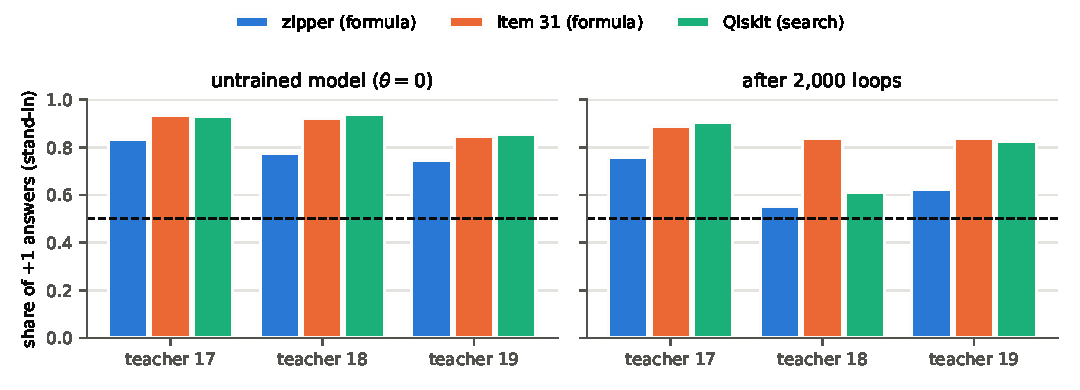
\includegraphics[width=\textwidth]{figures/qml_confounds_plus.pdf}
\caption{Share of $+1$ answers on the stand-in (shot-free), far teachers. Labels are balanced (dashed line, 0.5).
Left: the untrained model, identical in all arms; right: after 2{,}000 loops.}
\label{fig:plus}
\end{figure}

Two consequences. First, accuracy and loss can disagree for a structural reason: accuracy reads the sign and is
sensitive to $\delta$; cross-entropy reads the magnitude and rewards a large $\lambda$. An arm with a small $\lambda$
and no offset can win on accuracy and lose on loss, and the reverse. On the far teachers at 500 loops Qiskit had the
lowest stand-in cross-entropy of the three arms on teacher 18 (0.585, with 250 shots) and an accuracy of 0.568,
against the zipper's 0.635 and 0.711. Second, a gain measured as
``accuracy after training minus accuracy at $\theta = 0$'' does not cancel the offset when the offset saturates one
class: item 31 on teacher 19 gains $+0.068$ noiseless but $-0.020$ on the stand-in by 2{,}000 loops.

\textbf{Check:} report the share of each answer next to accuracy, and an offset-free measure (AUC, or the trained
model's noiseless accuracy).

\section{Confound 3: unequal shot fragility}
\label{sec:shots}

The zipper's output is shrunk more than item 31's on the twin, and the gap widens with depth ($\lambda$ 0.375 against
item 31's 0.398 at $L = 8$; 0.113 against 0.249 at $L = 20$; means over three teachers). To read the zipper's decisions with the
noise of 250 shots of item 31's, the device would need $4.8\times$ the shots at $L = 20$. In the declared data test
($L = 16$, 256 training points) the zipper's shot-free accuracy was 0.80--0.83 against item 31's 0.61--0.65; with the
run's 250 shots it was 0.70--0.74 against 0.63--0.64. From shot-free to 250 shots at 2{,}000 loops on the far
teachers the zipper lost 0.016, 0.017 and 0.046 and Qiskit, whose twin scale is the largest on the device day's
model, $-0.001$, 0.044 and $-0.007$. Item 31 lost 0.001, $-0.034$ and $-0.058$: for an arm with a saturating offset,
shot noise can \emph{raise} accuracy by randomising some of the answers the offset had fixed.

\textbf{Check:} report shot-free and shot-based accuracy, and the output scale, per arm; fix the shot count in the
declaration.

\section{Declared tests on teachers far from the start}

\subsection{Data and early learning, zipper against item 31 (angle 0.3; declared)}

Two earlier declared tests at angle 0.3 are summarised for completeness. In the data test (teachers 14--16, 2{,}000
loops) more training data was not the limit (256 against 64 points: WIN in 1 of 3 teachers for item 31, 0 of 3 for
the zipper), and the zipper's raw accuracy lead survived it (3 of 3; 0.804/0.610, 0.830/0.644, 0.818/0.652; Holm $p
\le 3\times10^{-13}$). Post hoc on the long training, on teacher 11 --- the one teacher that needed learning ---
item 31 read the untrained model out better ($\delta$ removed: 0.718 against 0.636), and in 500 loops the zipper
gained $+0.242$ against item 31's $+0.018$ (stand-in AUC $0.717 \to 0.957$ against $0.783 \to 0.864$). One teacher is
a hypothesis, not a result; the next test was declared to check it.

\subsection{Zipper against item 31 on far teachers (declared)}
\label{sec:fart}

Teachers 17, 18, 19 at angle 1.0; untrained noiseless accuracy 0.574, 0.640, 0.498. Rule A: shot-free stand-in
accuracy, zipper against item 31, McNemar, Holm over 6. Rule B: what training added, per point $g = \text{correct}
(\text{trained}) - \text{correct}(\theta = 0)$ per arm, Wilcoxon on $g_{\text{zipper}} - g_{\text{item 31}}$.

\begin{table}[h]
\centering
\small
\begin{tabular}{lcccc}
\toprule
 & \multicolumn{2}{c}{500 loops} & \multicolumn{2}{c}{2{,}000 loops} \\
teacher & A: zipper / item 31 & B: gain zipper / item 31 & A: zipper / item 31 & B: gain zipper / item 31 \\
\midrule
17 & 0.584 / 0.546 & $+0.008$ / $+0.008$ & 0.622 / 0.578 & $+0.046$ / $+0.040$ \\
18 & \textbf{0.776 / 0.538} & $\mathbf{+0.152}$ / $\mathbf{+0.018}$ & \textbf{0.780 / 0.636} & $+0.156$ / $+0.116$ \\
19 & 0.576 / 0.554 & $+0.076$ / $+0.020$ & \textbf{0.658 / 0.514} & $\mathbf{+0.158}$ / $\mathbf{-0.020}$ \\
\midrule
verdict & \multicolumn{2}{c}{A: no (1 of 3); B: no (1 of 3)} & \multicolumn{2}{c}{A: \textbf{yes} (2 of 3); B: no (1 of 3)} \\
\bottomrule
\end{tabular}
\caption{Far teachers, zipper against item 31 (stand-in, shot-free). Bold: WIN after Holm at $\alpha = 0.01$.}
\label{tab:fart}
\end{table}

\begin{itemize}
\item \textbf{Vanity:} at 2{,}000 loops the zipper is the more accurate (2 of 3); on teacher 18 at 500 loops by
$+0.24$.
\item \textbf{Essential:} the declared ``learns more'' (B) is not supported at either budget. Item 31 answered $+1$ on
84--94\,\% of the balanced points at every budget, so part of A's verdict is its offset. B's premise --- that the
offset cancels in the gain --- failed where the offset saturates (Section~\ref{sec:offset}).
\item \textbf{Post hoc:} the trained models themselves (noiseless accuracy, McNemar, Holm) differ in 1 of 3 teachers at
500 loops and 0 of 3 at 2{,}000. In noiseless gain the zipper learned the same on teacher 17 ($+0.056$ / $+0.064$),
faster on 18 ($+0.130$ / $+0.010$ at 500 loops) and more on 19 ($+0.142$ / $+0.068$).
\end{itemize}

\subsection{Formula against search: zipper against Qiskit on far teachers (declared)}
\label{sec:farq}

Same plans; the Qiskit arm was trained and verified anew, the zipper's records reused (identical test labels,
checked). Rule A as above; Rule B is the trained model's noiseless accuracy (declared to avoid B's flaw above). A
device run of the comparison was to be declared only if the power of one McNemar test at 300 points, simulated from
the stand-in with 250 shots, reached 0.8 in 2 of 3 teachers at one budget.

\begin{table}[h]
\centering
\small
\begin{tabular}{lcccc}
\toprule
 & \multicolumn{2}{c}{500 loops} & \multicolumn{2}{c}{2{,}000 loops} \\
teacher & A: zipper / Qiskit & B: zipper / Qiskit & A: zipper / Qiskit & B: zipper / Qiskit \\
\midrule
17 & 0.584 / 0.566 & 0.594 / 0.626 & 0.622 / 0.570 & 0.630 / 0.630 \\
18 & \textbf{0.776 / 0.554} & 0.770 / 0.764 & 0.780 / 0.778 & 0.786 / 0.818 \\
19 & 0.576 / 0.614 & 0.590 / 0.624 & \textbf{0.658 / 0.582} & 0.640 / 0.600 \\
\midrule
verdict & \multicolumn{2}{c}{A: neither (1 WIN); B: neither (0)} & \multicolumn{2}{c}{A: neither (1 WIN); B: neither (0)}
\\
\bottomrule
\end{tabular}
\caption{Far teachers, zipper (formula) against Qiskit (search). A: stand-in, shot-free; B: trained model, noiseless.
Bold: zipper WIN after Holm; there was no LOSS.}
\label{tab:farq}
\end{table}

\begin{figure}[h]
\centering
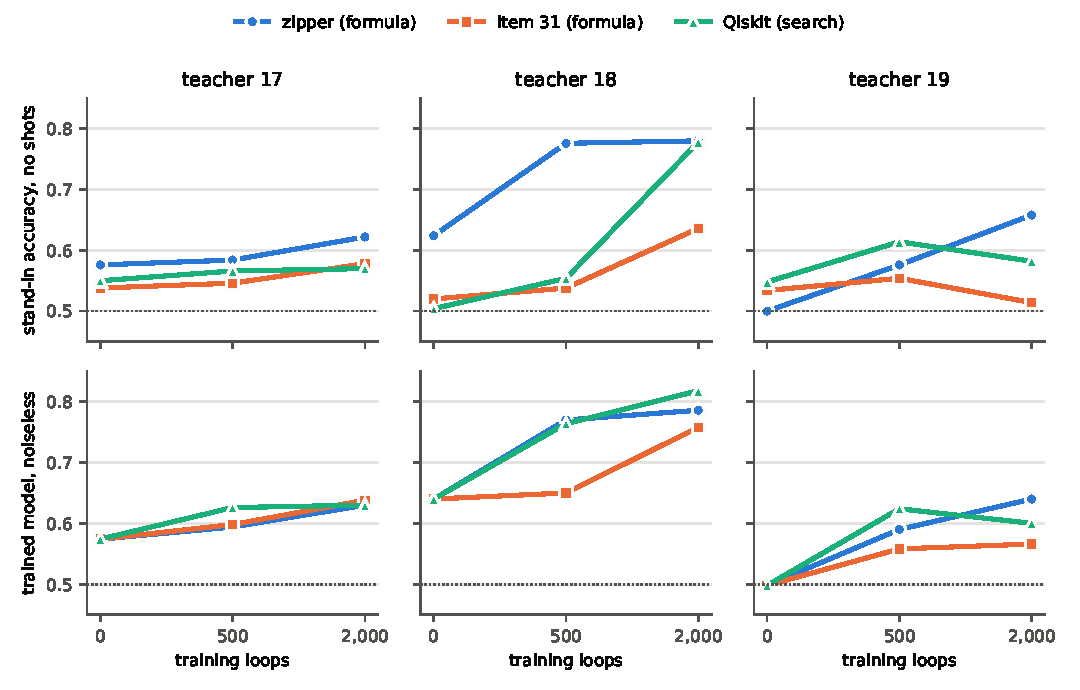
\includegraphics[width=\textwidth]{figures/qml_confounds_far.pdf}
\caption{Far teachers: accuracy at $\theta = 0$, 500 and 2{,}000 loops for the three arms. Top: stand-in, shot-free
(what the circuit delivers). Bottom: the trained model, noiseless (what was learned). At $\theta = 0$ the bottom row
is one point: all arms start from the same model.}
\label{fig:far}
\end{figure}

\begin{itemize}
\item \textbf{Vanity:} the zipper beats Qiskit on teacher 18 at 500 loops ($0.776$ against $0.554$, Holm
$p = 4\times10^{-14}$) with a third fewer CZ, a quarter of the duration and 4 fewer qubits.
\item \textbf{Essential:} by the declared rules neither compiler gives the more accurate classifier, and what they
learn cannot be told apart. A tie on one seed and three teachers is not a proof of equality. The device threshold
was met only on teacher 18 at 500 loops (power 0.96); by the declaration, no device time was spent.
\item \textbf{Reported:} Qiskit's offset persists after training ($+1$ on 81--93\,\% of points) except on teacher 18 at
2{,}000 loops (0.61), where its accuracy rose to 0.778. The twin predicts the zipper's circuit better than Qiskit's
(per-point rmse of $P(1)$, twin against stand-in: 0.008--0.014 against 0.016--0.055); at 500 loops Qiskit's stand-in
cross-entropy fell outside the twin's 99\,\% interval on two teachers. Stand-in AUC at 2{,}000 loops: 0.762/0.771,
0.910/0.909, 0.739/0.730.
\item \textbf{Cost:} the Qiskit arm took 4\,h\,51\,min on an H100 against the declared 1--1.5\,h; its trajectories
evolve 14 active qubits, a state $2^{14}/2^{10} = 16$ times larger than the zipper's. This is a simulation cost; on hardware, by the billing model TOQB uses
(0.036\,s per circuit plus 0.27\,ms and the circuit's duration per shot), 250 shots of a test point take about
$0.12$\,s for Qiskit's circuit and $0.11$\,s for the zipper's.
\end{itemize}

Before the run, the workplace instance of the project wrote eight predictions for this comparison. Five held
(Qiskit near chance at $\theta = 0$; AUC within 0.05; no consistent winner in what was learned; Qiskit less
shot-fragile; teacher 17 hard for every arm), two held in part (Qiskit's $+1$ share at least 0.80: 8 of 9 cells; the
twin at least 0.02 off on Qiskit's circuit: at $\theta = 0$, in 2 of 3 teachers at 500 loops, not at 2{,}000), and one failed: the zipper did not win raw accuracy at
2{,}000 loops in 2 of 3 teachers.

\subsection{A first hardware run of the zipper (preliminary; declared, report only)}
\label{sec:kingston}

After the tests above, the trained far-teacher models of both arms (2{,}000 loops, teachers 17--19) were sent to
hardware without retraining: one job on \texttt{ibm\_kingston} on 24 October 2026, the first 90 test points per
teacher and arm, 540 circuits of 250 shots, 42\,s of QPU time. Declared before submission as a report without a rule
(TOQB \path{prereg/drafts-2026-10-24/flow_c_note.md} and its amendment, which moved the job from
\texttt{ibm\_marrakesh}, paused for maintenance, to \texttt{ibm\_kingston}, chosen by queue length alone). Each arm was
compiled for the calibration fetched 36 minutes before submission, and its prediction was made with a twin built
from that calibration; the device recalibrated once in between, with unchanged values on all qubits of both arms.

\begin{table}[h]
\centering
\small
\begin{tabular}{p{5.6cm}p{3.6cm}p{4.6cm}}
\toprule
 & zipper (336 CZ, $10.8\,\mu$s) & Qiskit ($506$ CZ, $45.8\,\mu$s) \\
\midrule
device against the day's twin: scale / correlation & $1.00$ / $0.98$ & $-0.16$ / $-0.53$ \\
per measured qubit (teacher 17): correlation with the noiseless values & all 10: $0.81$--$0.99$ & 5: about 0; 3: $0.37$--$0.44$; 2 inverted \\
share of $+1$ answers, device / noiseless & $0.85$ / $0.79$--$0.83$ & $0.39$ / $0.83$--$0.87$ \\
\bottomrule
\end{tabular}
\caption{One job on \texttt{ibm\_kingston}, 90 points per teacher and arm. Scale and correlation: least-squares fit of
the device's $\langle Z\rangle$ per point on the twin's. The read-out qubit of Qiskit's circuits is one of the two
inverted ($-0.55$).}
\label{tab:kingston}
\end{table}

\begin{itemize}
\item \textbf{Vanity:} the device's ``accuracy'' is $0.85$--$0.87$ for the zipper and $0.37$--$0.47$ for Qiskit. It is
not an accuracy here: the test sets are ordered by label and the first 90 points are all of one class, an error in our
declaration found after the job. The column is the share of $+1$ answers and is not read.
\item \textbf{Essential:} the zipper's circuits ran as the twin of the day's calibration said, on every measured qubit;
on the device day (Section~\ref{sec:device}, \texttt{ibm\_marrakesh} with a twin from a 9-day-old calibration) the
twin had been off by up to $2.3\times$. Qiskit's circuits, on the same job, lost most of their signal and were inverted on the read-out
qubit. Not a software error as far as checked: Qiskit's own statevector of the submitted circuits agrees with the twin
(correlation $0.995$). A uniform static ZZ of 10\,kHz added to the twin does not reproduce the inversion; the cause is
not found.
\item \textbf{Not claimed:} one job, one device, 90 points of one label per cell, no arm comparison tested. Qiskit's
layout may have met a fault of that device and day; whether formula placement avoids such faults more often than a
calibration-aware search is a question for many jobs, not this one.
\end{itemize}

\section{Discussion}

\paragraph{What the formula buys.} On this classifier at $L = 16$, formula placement without calibration
was not distinguishable from calibration-aware search by either declared rule (one zipper WIN under rule A at each
budget, no LOSS), with 336 instead of 506 CZ and $11.7$ instead of $48.2\,\mu$s. How Qiskit's longer circuit keeps
up is not established; one possible reason, untested, is its calibration-aware choice of qubits: on the device day's
model its twin scale $\lambda$ is $2.7$ times the zipper's despite the longer circuit. The two routes reach
classifiers the tests could not tell apart, by different trades. Where the formula should pull ahead is where
duration and qubit count grow faster than good qubits can be found --- deeper or wider circuits --- and in
reproducibility, since the formula's circuit does not change with the day's calibration. Neither is shown here.

\paragraph{What the zipper does and does not do.} Against PSF-Zero's own earlier template, the zipper reads the model
out with a much smaller offset, and on the twin its noise acts as one uniform shrink. The twin predicts the zipper's
circuit about as well as item 31's, and better than Qiskit's. It
did not, by the declared test, learn more. Its smaller $\lambda$ costs shots, increasingly with depth.

\paragraph{The confounds are general.} None of the four effects is specific to PSF-Zero or Qiskit. Any comparison of
compilers, devices or noise levels through a trained classifier can be won by a readout offset, a near-start task, a
shot count that favours one output scale, or a device model off by a constant factor. Each was present in this
project's earlier results, and each changed a conclusion.

\section{Checklist for compiler comparisons through trained models}

\begin{enumerate}
\item Report the untrained model ($\theta = 0$) per arm on the test tier, and place teachers where learning is needed.
\item Report the share of each answer next to accuracy; an arm far from the label prior has an offset.
\item Report an offset-free measure: the trained model's noiseless accuracy, or AUC.
\item Report shot-free and shot-based accuracy and the output scale per arm; fix the shot count in advance.
\item Measure the device model's scale against hardware (per-point regression) before trusting predicted absolute
values.
\item Separate declared from post hoc results, and give the vanity and the essential number together.
\end{enumerate}

\section{Limitations}

\begin{itemize}
\item One training seed; three teachers per test; $n = 10$; $L = 16$ for the declared far-teacher tests.
\item All learning results are on simulators. The stand-in shares the twin's calibration base. The zipper has run on
hardware in one job only (Section~\ref{sec:kingston}), with 90 points of one label per cell.
\item The post hoc analyses were guided by earlier results; their $p$-values are descriptive.
\item The twin's scale was off by up to $2.3\times$ on hardware for PSF-Zero; shot costs derived from the twin's
$\lambda$ are therefore uncertain on hardware.
\end{itemize}

\section{Reproducibility}

All runs, records and scores are in the TOQB test bench (\url{https://github.com/TN-Holdings-LLC/TOQB}), each result folder with the declaration it was scored against and, where the run produced one, the zip's SHA-256: device day
\path{results/device-2026-10-22} (with \path{theta0_home}); long training \path{results/zip-long-2026-10-23};
data test \path{results/data-grad-2026-10-23}; depth sweep \path{results/zip-depth-2026-10-22}; noise sources
\path{results/lam-ablate-2026-10-22}; far teachers \path{results/far-teacher-2026-10-23} (declared in
\texttt{f5ed070}); zipper against Qiskit \path{results/far-qiskit-2026-10-23} (declared in \texttt{fe488cb}); the
\texttt{ibm\_kingston} job \path{results/flow-c-2026-10-24} (declared in \texttt{8f95fdd} and \texttt{f1a2575}, every
point in \path{points.csv}). The
compilers are Qiskit 2.5.2 and PSF-Zero \texttt{9f0d44e} for the far-teacher tests (\texttt{6269c4f} for the device
day, the depth sweep and the noise-source runs). The figures are computed from those records by
\path{docs/papers/qml_confounds_figures.py}.

\paragraph{Changes in version 1.2.} Section~\ref{sec:kingston} (the zipper's first hardware job, preliminary), one
sentence in the abstract, and the limitation on hardware updated. Nothing else changes.

\paragraph{Changes in version 1.1.} Section 2.2 now states how the zipper arm was built (TOQB's Python
implementation, identical to PSF-Zero a24's circuits); version 1 said both PSF-Zero arms were built by a24's Rust
builder. No number or verdict changes.

\begin{thebibliography}{99}

\bibitem{psfzero} TN Holdings, ``PSF-Zero: An Analytic Two-Qubit Gate Synthesizer Combined with a Verified,
Ordering-Aware Layout Search for Quantum Circuit Transpilation'', Version 2 (2026).
\url{https://github.com/TN-Holdings-LLC/psf-zero}

\bibitem{qiskit} A. Javadi-Abhari et al., ``Quantum computing with Qiskit'', arXiv:2405.08810 (2024).
\url{https://arxiv.org/abs/2405.08810}

\bibitem{perez2020} A. P\'erez-Salinas, A. Cervera-Lierta, E. Gil-Fuster, J. I. Latorre, ``Data re-uploading for a
universal quantum classifier'', Quantum 4, 226 (2020). \url{https://quantum-journal.org/papers/q-2020-02-06-226/}

\bibitem{wang2021} S. Wang et al., ``Noise-induced barren plateaus in variational quantum algorithms'', Nature
Communications 12, 6961 (2021). \url{https://arxiv.org/abs/2007.14384}

\bibitem{vovrosh2021} J. Vovrosh et al., ``Simple mitigation of global depolarizing errors in quantum simulations'',
Physical Review E 104, 035309 (2021).

\bibitem{urbanek2021} M. Urbanek et al., ``Mitigating depolarizing noise on quantum computers with noise-estimation
circuits'', Physical Review Letters 127, 270502 (2021).

\bibitem{nguyen2026} V.-Q.-M. Nguyen, T.-V. Truong, H.-L. Nguyen, T.-K. Le, ``Zero- versus infinite-temperature
damping in variational quantum circuits: feature scale, sampling cost, and frame gauge'', arXiv:2610.01466 (2026).
\url{https://arxiv.org/abs/2610.01466}

\bibitem{kashif2026a} M. Kashif, M. Shafique, ``Late breaking results: hardware-aware compilation reshapes
trainability in variational quantum circuits'', arXiv:2604.16527 (2026). \url{https://arxiv.org/abs/2604.16527}

\bibitem{kashif2026b} M. Kashif, M. Shafique, ``Beyond logical circuits: hardware-aware analysis of expressibility and
trainability in variational quantum algorithms'', arXiv:2605.25552 (2026). \url{https://arxiv.org/abs/2605.25552}

\bibitem{bowles2024} J. Bowles, S. Ahmed, M. Schuld, ``Better than classical? The subtle art of benchmarking quantum
machine learning models'', arXiv:2403.07059 (2024). \url{https://arxiv.org/abs/2403.07059}

\bibitem{ogorman2019} B. O'Gorman, W. J. Huggins, E. G. Rieffel, K. B. Whaley, ``Generalized swap networks for
near-term quantum computing'', arXiv:1905.05118 (2019). \url{https://arxiv.org/abs/1905.05118}

\bibitem{parella2025} T. Parella-Dilm\'e, J. S. Kottmann, A. Ac\'in, ``Swap network augmented ans\"atze on arbitrary
connectivity'', arXiv:2507.23679. \url{https://arxiv.org/abs/2507.23679}

\end{thebibliography}

\end{document}
